% ICSIE 2027 draft (Plan A): ChineseEEG lexical encoding. Revised 2026-11-03 for Shimamura's five points (2026-10-31).
% Style pass 2026-11-04: short sentences, passive voice, no clause chains with , ; : in prose, no overclaiming words.
% Not sent; Shimamura approves first.
% Template: ICSIE 2027 Download Center "LaTeX-Templates.zip" (ACM acmart, sigconf).
% Build: pdflatex main && bibtex main && pdflatex main && pdflatex main
% Numbers, tables and figures: numbers.tex, table_*.tex, fig_*.pdf <- scripts/chineseeeg_paper_assets.py
%   runs/chineseeeg_regression_locked_corrected paper runs/locked_first_read_old_onsets runs/chineseeeg_regression_locked_nulls
% Plan: lab01/.claude/prds/exp-chineseeeg-overlap-regression-2026-10.md.
\documentclass[sigconf]{acmart}
\usepackage{booktabs}
\usepackage{tikz}
\usetikzlibrary{positioning,arrows.meta,fit,backgrounds,calc}
\DeclareRobustCommand{\guardmark}[1]{\tikz[baseline=(g.base)]\node[circle, fill=red!70!black, text=white, font=\scriptsize\bfseries, inner sep=0.6pt, minimum size=3.4mm](g){#1};}

\AtBeginDocument{\providecommand\BibTeX{{Bib\TeX}}}

\setcopyright{acmlicensed}
\copyrightyear{2027}
\acmYear{2027}
\acmDOI{XXXXXXX.XXXXXXX}
\acmConference[ICSIE 2027]{2027 15th International Conference on Software and Information Engineering}{January 15--17, 2027}{Tokyo, Japan}
\acmISBN{978-1-4503-XXXX-X/2027/01}

\newcommand{\nSubj}{7}
\newcommand{\charsMin}{90\,040}
\newcommand{\charsMax}{96\,251}
\newcommand{\testCharsMin}{14\,248}
\newcommand{\testCharsMax}{17\,116}
\newcommand{\runsMin}{22}
\newcommand{\runsMax}{24}
\newcommand{\condL}{2.3}
\newcommand{\dRmean}{5.1}
\newcommand{\dRlo}{1.9}
\newcommand{\dRhi}{9.4}
\newcommand{\dRmin}{0.2}
\newcommand{\dRmax}{16.8}
\newcommand{\dRpos}{7}
\newcommand{\dRp}{0.0078}
\newcommand{\pctNmin}{0.001}
\newcommand{\pctNmax}{0.04}
\newcommand{\pctNeyemin}{0.002}
\newcommand{\pctNeyemax}{0.17}
\newcommand{\rNmin}{0.29}
\newcommand{\rNmax}{0.52}
\newcommand{\rNeyemin}{0.04}
\newcommand{\rNeyemax}{0.11}
\newcommand{\nullNeg}{6}
\newcommand{\nullMin}{-4.3}
\newcommand{\nullMax}{0.0}
\newcommand{\permFloor}{5}
\newcommand{\zmin}{0.1}
\newcommand{\zmax}{11.4}
\newcommand{\strokesMean}{8.4}
\newcommand{\strokesPos}{6}
\newcommand{\strokesP}{0.016}
\newcommand{\embMean}{0.8}
\newcommand{\embPos}{6}
\newcommand{\embP}{0.055}
\newcommand{\dRfrontal}{1.2}
\newcommand{\dRposterior}{6.4}
\newcommand{\postGtFront}{5}
\newcommand{\surpPeak}{297}
\newcommand{\surpNeg}{7}
\newcommand{\freqPeak}{234}
\newcommand{\freqPosAtPeak}{6}
\newcommand{\looFreqMean}{3.2}
\newcommand{\looFreqPos}{6}
\newcommand{\looSurpMean}{2.8}
\newcommand{\looSurpPos}{7}
\newcommand{\strokesOverLex}{1.6}
\newcommand{\nullsShuffleFloor}{5}
\newcommand{\nullsShuffleFloorRe}{5}
\newcommand{\nullsCircularFloor}{4}
\newcommand{\nullsCircularFloorRe}{5}
\newcommand{\nullsReMeanMin}{-0.5}
\newcommand{\nullsReMeanMax}{0.3}
\newcommand{\nullsCircNeg}{6}
\newcommand{\nullsReNarrower}{7}
\newcommand{\nullsMaxP}{0.60}
\newcommand{\nullsFloorAllMin}{4}

\newcommand{\dR}{\Delta R}
\newcommand{\tenm}[1]{#1\times10^{-5}}

\begin{document}

\title[Lexical Effects in Continuous Reading EEG]{A Small and Consistent Lexical Effect in Continuous Chinese Reading EEG under Overlap-Corrected Encoding with Run-Level Splits and Training-Only Penalty Selection}

\author{Khin Pyae Phyo San}
\orcid{0009-0000-3299-2065}
\email{khin.s.038@ms.saitama-u.ac.jp}
\affiliation{%
  \department{Department of Information and Computer Science}
  \institution{Saitama University}
  \city{Saitama}
  \postcode{338-8570}
  \country{Japan}}

\author{Amy Lynn Latt}
\email{ami.l.l.783@ms.saitama-u.ac.jp}
\affiliation{%
  \department{Department of Information and Computer Science}
  \institution{Saitama University}
  \city{Saitama}
  \postcode{338-8570}
  \country{Japan}}

\author{Tetsuya Shimamura}
\orcid{0000-0002-7874-3467}
\email{shima@mail.saitama-u.ac.jp}
\affiliation{%
  \department{Department of Information and Computer Science}
  \institution{Saitama University}
  \city{Saitama}
  \postcode{338-8570}
  \country{Japan}}

\renewcommand{\shortauthors}{K. P. P. San, A. L. Latt, and T. Shimamura}

\begin{abstract}
Claims that language can be decoded from scalp EEG are hard to check. A pipeline that reports chance cannot tell a weak signal from a broken analysis. A pipeline that reports success may be using position or eye movements or overlapping responses to neighbouring words. An encoding pipeline for continuous reading EEG was built to detect a reported effect under controlled conditions before it is used for anything new. An overlap-corrected linear model (finite impulse response with banded ridge) is fitted to the public ChineseEEG corpus. In this corpus two novels were read one highlighted character at a time. Character onsets are derived from the row markers and from the published presentation code. Character onset and position in the row are modelled as nuisance together with row boundaries and stroke count and eleven periocular channels. Character log frequency and language-model surprisal together form the tested feature space. Runs are split before fitting. Penalties are chosen inside the training runs only. A hypothesis fixed in a version-controlled plan is tested on held-out runs that were not used to tune this model. The test was scored twice. The second read followed a correction of the onset formula found in review. Both reads are reported and agree. In all \nSubj{} of 10 readers who passed a timing check the held-out EEG prediction correlation was increased by the lexical feature space (one-sided Wilcoxon $p=\dRp$ with mean $\dR=\tenm{\dRmean}$ and 95\,\% CI $\tenm{\dRlo}$ to $\tenm{\dRhi}$). At group level the gain is larger over posterior than over frontal channels. The surprisal kernel is negative at 300--500\,ms in \surpNeg{} of \nSubj{} readers. This is a descriptive pattern consistent with an N400-like response. The increase is consistent but very small. It is at most \pctNmax\,\% of the prediction correlation of the nuisance model. This is a ratio of correlations and not explained variance. The safeguards are described and effect sizes are reported so that later analyses of the same data have a reference effect obtained with the same onsets and split.
\end{abstract}

\begin{CCSXML}
<ccs2012>
<concept><concept_id>10010405.10010444.10010087</concept_id><concept_desc>Applied computing~Computational biology</concept_desc><concept_significance>300</concept_significance></concept>
<concept><concept_id>10010147.10010257.10010258.10010259.10010264</concept_id><concept_desc>Computing methodologies~Supervised learning by regression</concept_desc><concept_significance>500</concept_significance></concept>
</ccs2012>
\end{CCSXML}
\ccsdesc[300]{Applied computing~Computational biology}
\ccsdesc[500]{Computing methodologies~Supervised learning by regression}

\keywords{EEG, reading, encoding model, surprisal, word frequency, overlap correction, data leakage, reproducibility}

\maketitle

\section{Introduction}
Recent work maps non-invasive brain recordings to language-model representations~\cite{tang2023semantic,defossez2023decoding}. For non-invasive recordings several such results shrink once shortcuts are controlled. Non-robust evaluation and overlooked confounds can produce apparent brain--model alignment~\cite{hadidi2026spurious}. Part of what retrieval models use can be traced to stimulus timing such as word duration~\cite{zhang2026decoding}. Controls create a second problem. When a controlled decoder scores at chance it cannot be told whether the brain signal is absent from the recording or whether the analysis is unable to find any signal.

One answer is a positive control. This is an effect that has been reported many times and that the same pipeline must detect under the same rules. For reading the lexical effects of word frequency~\cite{zeng2025coregistration} and predictability have been reported widely. Words that are less expected from context evoke a larger centro-parietal negativity around 300--500\,ms. This is the N400~\cite{kutas2011thirty}. Language-model surprisal predicts this response in sentence reading~\cite{frank2015erp} and in Mandarin reading~\cite{salicchi2025metric}. Related context measures predict EEG and MEG responses to narrative speech~\cite{broderick2018semantic,heilbron2022hierarchy}.

This idea is applied to ChineseEEG~\cite{mou2024chineseeeg}. This public corpus holds about 100\,000 characters of novel reading per participant. Each character is shown for a fixed time. This makes the corpus suitable for character-locked analysis. Two properties of the corpus make shortcuts easy. Characters follow each other about every 0.43\,s. The response to one character therefore overlaps the next. The eyes of the reader follow a moving highlight. Eye movements are therefore time-locked to every character.

One question was fixed in a written plan before any regression code existed. \emph{Once overlap, row position, row boundaries, visual complexity and periocular signals are modelled, do character frequency and surprisal together still increase held-out prediction correlation?} The contributions are listed below.
\begin{itemize}
\item An overlap-corrected banded-ridge encoding pipeline for continuous reading EEG. It uses run-level splits, feature scaling fitted on training runs only, and penalty selection inside the training runs only. A timing gate excludes readers before any model is fitted and character onsets are derived from the presentation code and the row markers (Section~\ref{sec:data}).
\item A pre-specified test on held-out runs that were not used to tune this model. The test was scored before and after an onset correction. The lexical feature space increased prediction correlation in \dRpos{} of \nSubj{} readers in both reads (Section~\ref{sec:results}).
\item An effect-size report whose items were fixed before the test. The items are per-reader gains, gains relative to the nuisance model, permutation nulls, channel distribution and kernel latency. The reported increase is consistent but very small.
\end{itemize}

\section{Related Work}
\textbf{Lexical effects in EEG.} The N400 tracks how expected a word is~\cite{kutas2011thirty}. Surprisal from a language model predicts N400 amplitude in sentence reading~\cite{frank2015erp} and in Chinese materials~\cite{salicchi2025metric}. In natural Chinese reading character and word frequency modulate fixation-related potentials~\cite{zeng2025coregistration}. Continuous speech studies relate context measures to EEG and MEG with temporal response functions~\cite{broderick2018semantic,heilbron2022hierarchy,crosse2016mtrf}.

\textbf{Overlap correction.} When stimuli follow each other faster than the brain response decays the averaging of epochs mixes neighbouring responses. Regression-based deconvolution fits one kernel per event type jointly over the continuous signal and separates them~\cite{smith2015regression,ehinger2019unfold}. In natural reading the same approach is used to model eye-movement events and fixation-related potentials~\cite{dimigen2011coregistration,dimigen2021regression,li2024parafoveal}. In banded ridge regression each feature space is given its own penalty. A weak space is then not drowned out by a strong one~\cite{duprelatour2022banded}.

\textbf{Shortcuts in brain--language mapping.} Compact convolutional decoders are the usual choice for non-invasive speech EEG~\cite{san2026comparative}. Non-robust methods and overlooked confounds can inflate brain--model alignment~\cite{hadidi2026spurious}. Part of what non-invasive retrieval models use can be traced to stimulus timing rather than meaning~\cite{zhang2026decoding}. On ChineseEEG character-level EEG segments have been aligned with a language model for text generation~\cite{lu2025eeg2textcn}. That study does not report how character onsets were set. Most other analyses work at row or sentence level. For example band power per row has been related to contextual-embedding features~\cite{wang2025contextual}. No study known to us tests character-level features against overlap and position and eye signals on held-out runs.

\section{Data}
\label{sec:data}
\textbf{Corpus.} ChineseEEG (OpenNeuro ds004952 v1.2.2)~\cite{mou2024chineseeeg} contains 128-channel recordings (EGI HydroCel net) of ten participants. Two Chinese novels were read silently. \emph{The Little Prince} has 7 runs and \emph{Garnett Dream} has 18 runs. Each screen shows up to three rows. Within a row one character at a time turns red. The preprocessed 0.5--30\,Hz derivative of the dataset authors is used. In that derivative bad channels were interpolated and ocular and cardiac components were removed by independent component analysis. The data were then re-referenced to the average of all channels. All topographies in this paper are therefore average-referenced. The first \emph{Little Prince} run is dropped because its row markers do not match its text.

\textbf{Character onsets.} Only the start (ROWS) and the end (ROWE) of each row are marked in the recordings. Punctuation is never highlighted. The dataset paper gives 0.35\,s per character. The published presentation script (\texttt{play\_novel.py} in the repository of the dataset authors) was read to establish what the markers mean. Each highlighted character is one PsychoPy routine of \texttt{shift\_time} $= 0.35$\,s. ROWS is sent after the stimuli for the first character are built and immediately before its routine. ROWS is therefore the onset of character~1. ROWE is sent after the routine of the last highlighted character. ROWE is therefore the offset of character~$n$ and not its onset. This corpus was recorded with the eye tracker. In that loop the routine timer is reset after the text stimuli are rebuilt for every character. Each character therefore lasts 0.35\,s plus the rebuild time $\delta$. The row duration is $n\,(0.35 + \delta) - \delta$. The markers agree with this reading. Over 22\,298 rows of two participants least squares gives duration $= 0.427\,n - 0.086$\,s (residual SD 0.10\,s). The slope and the intercept both give $\delta \approx 0.08$\,s. The loop without the eye tracker would give slope 0.35 and intercept 0. Pauses and scrolling fall outside the markers. The step between successive onsets is therefore the row span minus the display of the last character divided by the $n-1$ intervals between $n$ onsets.
\[
t_k = t_\text{ROWS} + k \, \frac{t_\text{ROWE} - t_\text{ROWS} - 0.35}{n - 1}, \qquad k = 0, \dots, n-1 .
\]
Rows whose span per character falls outside 0.30--0.60\,s are dropped. The first version of this analysis divided the span by $n$. That formula places the $k$-th onset early by about $k \times 8$\,ms. The error reaches 70\,ms at the end of a ten-character row and is 35\,ms on average. A fixed 0.35\,s pace would drift by up to 0.7\,s. Section~\ref{sec:decided} states which results used which formula. The rebuild time varies between characters and cannot be recovered without the eye-tracking stream. Single onsets therefore keep an uncertainty of roughly 10--30\,ms plus one monitor frame. The script that fits the row-duration model is in the repository.

\textbf{Timing gate.} Interpolated onsets are only useful if the EEG follows them. Before any model was fitted each participant had to show a character-locked occipital response. Only training and validation runs were used. The response is the grand-average EEG of seven occipital channels (E70 E71 E74 E75 E76 E82 E83) over characters at row position 5 or later. Its amplitude is the peak-to-trough value over 0--0.4\,s after onset. The same amplitude was computed for two comparison onset sets. One used the fixed 0.35\,s pace. The other shifted every onset by a random amount drawn uniformly within half a character step (jittered onsets). Three criteria were applied. (i) The amplitude with the measured pace exceeded three times the jittered amplitude. (ii) It exceeded the fixed-pace and the jittered amplitudes. (iii) A logistic regression on 0--0.4\,s EEG of all channels told the first character of a row apart from the others with a run-wise cross-validated AUC above 0.55. Criterion (iii) is a data check because the first onset is marked exactly. Table~\ref{tab:gate} gives the values of all ten participants. Its columns Row and Fixed and Jit.\ are the occipital peak-to-trough amplitudes ($\mu$V) with the measured pace and the fixed 0.35\,s pace and the jittered onsets. AUC is the first-character data check and Pass applies criteria (i) to (iii). The left block of the table selected the readers and the right block is the re-run after the test. Seven passed (S04 and S06 to S10 and S14). S05 and S15 failed (ii) and S13 failed (i). Criterion (i) was changed during the gate. The first rule required a visual peak at 80--200\,ms. S04 and S05 were checked first under that rule. S04 failed it. The rule was found to pick a trough rather than the peak. It was then replaced by criterion (i) before the other eight participants were checked and before any model was fitted. S04 passes the new rule. S05 fails both rules. The gate was applied with the span-over-$n$ onsets and the reader set was fixed before the test. The gate was re-run with the corrected onsets after the test. All seven originally selected participants also passed with the corrected onsets. The response of every one of them is larger with the corrected onsets (by 4--16\,\%). This is consistent with a better alignment. S13 additionally met the criteria after correction (0.62\,$\mu$V against three times 0.20\,$\mu$V) but was not included because the participant set had been fixed before the test results were examined. This gives \charsMin--\charsMax{} character events in \runsMin--\runsMax{} runs per participant.

\begin{table}
\caption{Timing gate for all ten participants.}
\label{tab:gate}
\footnotesize
\setlength{\tabcolsep}{3.5pt}
\begin{tabular}{lrrrrlrrl}
\toprule
 & \multicolumn{5}{c}{Span$/n$ onsets (selection)} & \multicolumn{3}{c}{Corrected onsets} \\
\cmidrule(lr){2-6} \cmidrule(lr){7-9}
Reader & Row & Fixed & Jit. & AUC & Pass & Row & Jit. & Pass \\
\midrule
S04 & 3.71 & 0.40 & 0.37 & 0.82 & yes & 3.84 & 0.46 & yes \\
S05 & 0.77 & 0.91 & 1.12 & 0.65 & no & 0.90 & 0.95 & no \\
S06 & 2.50 & 0.46 & 0.20 & 0.77 & yes & 2.65 & 0.17 & yes \\
S07 & 3.53 & 0.27 & 0.19 & 0.87 & yes & 3.70 & 0.29 & yes \\
S08 & 2.01 & 0.20 & 0.34 & 0.74 & yes & 2.28 & 0.30 & yes \\
S09 & 1.67 & 0.15 & 0.09 & 0.87 & yes & 1.89 & 0.09 & yes \\
S10 & 1.45 & 0.13 & 0.15 & 0.87 & yes & 1.68 & 0.16 & yes \\
S13 & 0.53 & 0.17 & 0.21 & 0.67 & no & 0.62 & 0.20 & yes \\
S14 & 3.05 & 1.03 & 0.60 & 0.83 & yes & 3.40 & 0.65 & yes \\
S15 & 2.07 & 2.17 & 1.28 & 0.74 & no & 2.42 & 1.94 & no \\
\bottomrule
\end{tabular}

\end{table}

\textbf{Lexical features.} Character log frequency is taken from the SUBTLEX-CH norms~\cite{cai2010subtlex}. 99.7\,\% of character tokens are covered. Character surprisal is taken from a Chinese GPT-2 with one token per character (\nolinkurl{uer/gpt2-chinese-cluecorpussmall}~\cite{zhao2019uer}). 0.2\,\% of the characters are unknown to it. The preceding text of the same run is used with punctuation included in sliding windows of 512 characters. Both features were computed from the text alone and were fixed before any EEG was fitted. Missing values are set to the training mean with a flag. The variance inflation factors of frequency and surprisal and stroke count and position were all below 1.3. The condition number of the lexical block was at most \condL.

\section{Method}
\label{sec:method}
\subsection{Encoding model}
EEG is band-passed at 0.5--8\,Hz (zero-phase FIR in MNE-Python~\cite{gramfort2013mne}). It is resampled to 64\,Hz and robust-$z$-scored per run and clipped at $\pm5$. The 117 non-periocular channels are the targets. Each event type enters a finite impulse response design with 58 lags from $-94$ to $797$\,ms. The design is fitted jointly over each run. The responses to character $k$ and to character $k+1$ are therefore estimated together rather than averaged into one epoch~\cite{smith2015regression,ehinger2019unfold}. The design has four bands. Each band has its own ridge penalty~\cite{duprelatour2022banded}.
\begin{description}
\item[C (nuisance events)] Character onset. Position in the row. First-in-row flag. Stroke count and its missing flag. Missing flags for the lexical features. Row start. Row end.
\item[eye (nuisance signals)] The 11 periocular channels as continuous regressors with lags $-0.1$ to $0.1$\,s.
\item[L (tested)] Log frequency and surprisal. Both are $z$-scored with the mean and standard deviation (SD) of the training-run text.
\item[E (exploratory)] The first ten principal components of static BERT character vectors~\cite{devlin2019bert}. The principal component analysis (PCA) is fitted on training-run text.
\end{description}
The nuisance model N contains C and eye. The tested model adds L. Two further models serve as diagnostics. One is N without stroke count. The other is N without the eye band.

\subsection{Evaluation protocol}
Runs are split by their order. The run at 0-based position $i$ in the fixed run list belongs to group $i \bmod 5$. Groups 0--3 are training data (19--20 runs per reader). Group 4 is the locked test set. It holds \emph{Garnett Dream} 5 and 10 and 15 and \emph{Little Prince} 3 (\testCharsMin--\testCharsMax{} characters). One reader (S09) has no recording of \emph{Little Prince} 3 and is tested on three runs. Penalties are searched jointly over a per-band grid by leave-one-group-out within groups 0--3 only. The grid is $10^1$--$10^9$ for C and eye and $10^1$--$10^7$ for L and E. An L band whose best penalty is the grid maximum counts as switched off and scores $\dR = 0$.

The primary measure is
\[
\dR = \tfrac{1}{117}\textstyle\sum_{c} \bigl[r_c(\text{N+L}) - r_c(\text{N})\bigr],
\]
which is the mean over channels of the gain in Pearson correlation between predicted and recorded held-out EEG. The hypothesis H1 is $\dR > 0$. It is tested with a one-sided Wilcoxon signed-rank test over the seven readers at $\alpha = 0.05$ (zeros split should a band be switched off). With $n = 7$ the smallest attainable $p$ is $1/128 = 0.0078$. Frequency and surprisal are added as one band. The test therefore speaks for the two-feature lexical space and not for either feature on its own.

Two further checks were fixed before the test. A within-run permutation null shuffles the lexical values across the characters of each run 200 times per reader (seed = reader number). Frequency and surprisal are shuffled together as pairs. Their mutual correlation is therefore kept. Onsets and the nuisance design and the penalties chosen for the real lexical values are kept as well. Hence $p = (1 + \#\{\dR_\text{perm} \ge \dR\})/201$ asks whether the real values predict better than values with the same marginal distribution placed on the wrong characters under penalties tuned to the real values. The null assumes exchangeability of the lexical values within a run. It breaks their serial order and their relation to position and stroke count. Penalties favourable to the real values can make the surrogate gains negative. A structure-preserving null and penalty re-selection for the surrogates were added in review after the test. They are reported as post hoc checks (Table~\ref{tab:nulls}). An effect-size rule requires that the per-reader gains with a bootstrap 95\,\% CI are reported with the $p$-value. The gains relative to the accuracy of the nuisance model and the channels carrying the gain and the sign and latency of the lexical kernels are required as well. How these items are measured was set in a script written after the locked run. The choices are the frontal and posterior quarters of the channels by their anterior--posterior position and the global-field-power peak and the 300--500\,ms window and 10\,000 bootstrap draws over readers. Figs.~\ref{fig:kernels}--\ref{fig:topo} and the channel results depend on these choices.

\subsection{Leakage guards and implementation}
Figure~\ref{fig:pipeline} shows where test data could leak into fitting and the safeguard placed at each point. Each safeguard is enforced in code and checked by an automatic test or record. The first guard is the timing gate. Onsets follow the measured pace of each row and readers whose EEG does not follow them are excluded before any fit. The second guard is the split by whole runs. The fitting code raises an error if a run appears on both sides. The third guard keeps feature scaling and PCA on training-run text only. The fourth guard fits from summed per-run statistics that are tested to equal ordinary ridge on the stacked data. The fifth guard chooses penalties inside the training runs. A lexical band at the largest penalty counts as switched off and scores exactly zero. The sixth guard keeps development code from loading the locked runs. The launcher writes a marker with the code version each time they are loaded. This happened three times in this paper (two reads and one surrogate pass as stated in Section~\ref{sec:decided}). Filtering and robust scaling are done per run and no statistic crosses runs. One implementation choice makes the analysis feasible on a workstation. The design for one reader (about 2.5 million samples $\times$ 1\,361 columns) is never held in memory. Each run is reduced to its sufficient statistics $X^\top X$ and $X^\top Y$ and the column and target sums and squares. Fits and penalty searches and held-out correlations are computed from sums of these per-run blocks. Held-out $r$ is computed from the per-run sums without approximation. Each per-group statistic block is a $1\,361 \times 1\,361$ matrix so memory does not grow with recording length. On one CPU the locked run took about 50 minutes per reader including the 200 permutations.

\begin{figure*}[t]
\centering
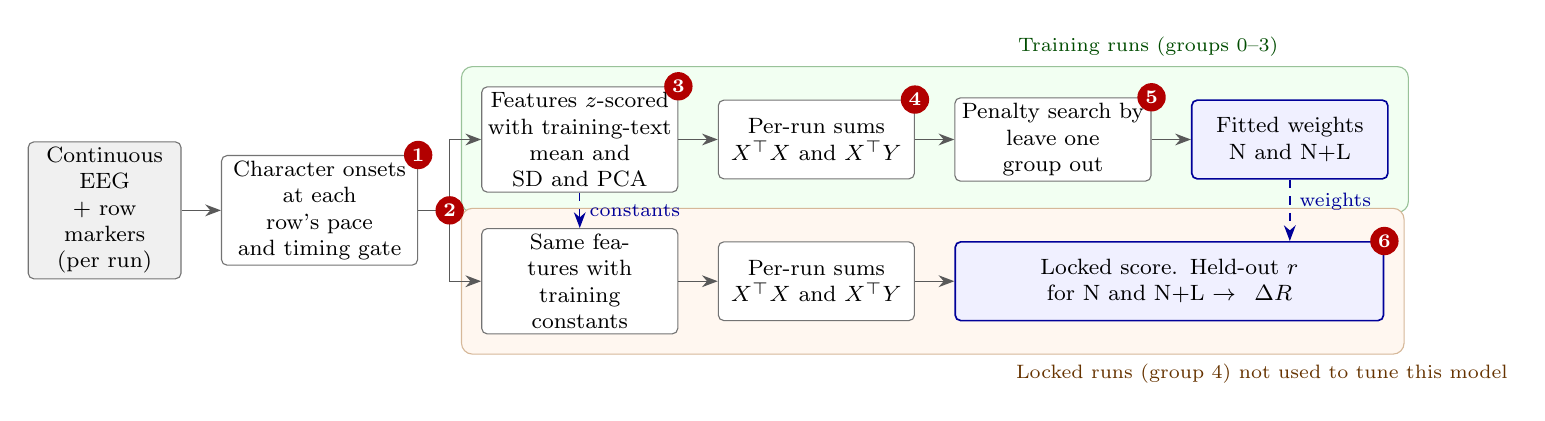
\begin{tikzpicture}[
  font=\footnotesize, node distance=4mm and 5mm,
  box/.style={draw=black!55, rounded corners=2pt, fill=white, align=center, minimum height=10mm, text width=23.5mm, inner sep=2pt},
  data/.style={box, fill=black!6},
  res/.style={box, draw=blue!60!black, fill=blue!6, line width=0.6pt},
  flow/.style={-{Stealth[length=2mm]}, black!65, line width=0.5pt},
  pass/.style={-{Stealth[length=2mm]}, blue!60!black, dashed, line width=0.5pt},
  guard/.style={circle, fill=red!70!black, text=white, font=\scriptsize\bfseries, inner sep=0.6pt, minimum size=3.6mm},
  lane/.style={rounded corners=4pt, inner sep=2.5mm}]
\node[data, text width=18mm] (raw) {Continuous EEG\\+ row markers\\(per run)};
\node[box, right=of raw] (onset) {Character onsets\\at each row's pace\\and timing gate};
\node[box, right=8mm of onset, yshift=9mm] (tfeat) {Features $z$-scored\\with training-text\\mean and SD and PCA};
\node[box, right=of tfeat] (tstat) {Per-run sums\\$X^\top X$ and $X^\top Y$};
\node[box, right=of tstat] (search) {Penalty search by\\leave one group out};
\node[res, right=of search] (weights) {Fitted weights\\N and N+L};
\node[box, right=8mm of onset, yshift=-9mm] (lfeat) {Same features with\\training constants};
\node[box, right=of lfeat] (lstat) {Per-run sums\\$X^\top X$ and $X^\top Y$};
\node[res, right=of lstat, text width=53mm] (score) {Locked score. Held-out $r$ for N and N+L $\rightarrow \Delta R$};
\begin{scope}[on background layer]
\node[lane, fill=green!5, draw=green!40!black!40, fit=(tfeat)(weights), label={[font=\scriptsize, text=green!30!black]above right:Training runs (groups 0--3)}] (trainlane) {};
\node[lane, fill=orange!6, draw=orange!60!black!40, fit=(lfeat)(score), label={[font=\scriptsize, text=orange!40!black]below right:Locked runs (group 4) not used to tune this model}] (locklane) {};
\end{scope}
\draw[flow] (raw) -- (onset);
\draw[flow] (onset.east) -- ++(4mm,0) |- (tfeat.west);
\draw[flow] (onset.east) -- ++(4mm,0) |- (lfeat.west);
\draw[flow] (tfeat) -- (tstat); \draw[flow] (tstat) -- (search); \draw[flow] (search) -- (weights);
\draw[flow] (lfeat) -- (lstat); \draw[flow] (lstat) -- (score);
\draw[pass] (tfeat.south) -- node[right, font=\scriptsize, text=blue!60!black]{constants} (lfeat.north);
\draw[pass] (weights.south) -- node[right, font=\scriptsize, text=blue!60!black, pos=0.35]{weights} (weights.south |- score.north);
\node[guard] at (onset.north east) {1};
\node[guard] at ($(onset.east)+(4mm,0)$) {2};
\node[guard] at (tfeat.north east) {3};
\node[guard] at (tstat.north east) {4};
\node[guard] at (search.north east) {5};
\node[guard] at (score.north east) {6};
\end{tikzpicture}
\caption{Data flow of the pipeline for one reader with the six safeguards against inflated results marked in red.}
\label{fig:pipeline}
\end{figure*}

\subsection{Analysis timeline and disclosures}
\label{sec:decided}
The plan and hypothesis and split were committed before any regression code existed. The timing gate had been run earlier for the retrieval analysis. Its first criterion was changed after S04 had failed the original latency rule (Section~\ref{sec:data}). A first development run on groups 0--3 (0.5--30\,Hz) gave no clear lexical or stroke gain. In that run the nuisance model was dominated by the periocular regressors. Before any locked data were read the band-pass was therefore lowered to 0.5--8\,Hz to suit the slow N400-range response. The clip was added. The eye band was separated from C. The nuisance penalty grid was widened. Text-derived constants were fixed per split. A second development run with these settings gave a lexical gain in 7/7 readers. The locked settings were then fixed and the locked test was scored (first read on 2026-10-31). The onsets were at $t_\text{ROWS} + k\,(t_\text{ROWE}-t_\text{ROWS})/n$.

In review the advisor asked why the pace was 0.42\,s rather than 0.35\,s and whether the span should be divided by $n$ or $n-1$. The verification in Section~\ref{sec:data} answered this from the presentation code and the markers. The first formula was found early by up to 70\,ms. The formula was corrected. The development folds were re-run with the same picture as before (lexical gain in 7/7 readers with a negative strokes control and a null embedding gain). The locked test was scored a second time with the corrected onsets and otherwise identical settings (second read on 2026-11-03). Nothing else was changed between the reads. The first read was not used to choose anything. All numbers and tables and figures in this paper come from the second read. Table~\ref{tab:reads} sets the two reads side by side. The first used onsets at span$/n$ (2026-10-31) and the second the corrected onsets of Section~\ref{sec:data}. Only the onset formula differs. Its means are in units of $10^{-5}$. The outputs of both are in the repository. After the second read the locked runs were loaded a third time (2026-11-03) only to build the surrogates of the post hoc nulls in Table~\ref{tab:nulls}. That pass fits the same models with the same penalties. The asset script checks that its observed gains equal those of the second read before the table is written.

A second disclosure applies to the test runs. Before this study their EEG had been read by a separate character-identity retrieval analysis with a different model and hypothesis. Its pre-specified tests found a small gain from EEG beyond neighbouring characters and row position (under one percentile point in 7/7 readers) and beyond the periocular channels (6/7 readers). The EEG decoder alone was not above chance on these runs. That result motivated the present plan. The plan was written afterwards to test a reported effect with a different model. The test runs were therefore not used to tune this model. They had been analysed before. ``Held out'' in this paper means held out from the development of the encoding model and not never analysed.

\section{Results}
\label{sec:results}
\begin{table}
\caption{Locked test per reader.}
\label{tab:subjects}
\small
\begin{tabular}{lrrrrrr}
\toprule
Reader & $r$(N) & $r$(N$-$eye) & $\Delta R$ & \% & $z$ & $p$ \\
\midrule
S04 & 0.394 & 0.088 & 0.2 & 0.001 & 0.1 & 0.438 \\
S06 & 0.353 & 0.036 & 1.4 & 0.004 & 1.4 & 0.109 \\
S07 & 0.415 & 0.110 & 7.9 & 0.019 & 7.5 & 0.005 \\
S08 & 0.291 & 0.075 & 2.5 & 0.009 & 3.3 & 0.005 \\
S09 & 0.435 & 0.103 & 3.9 & 0.009 & 4.6 & 0.005 \\
S10 & 0.418 & 0.098 & 16.8 & 0.040 & 11.4 & 0.005 \\
S14 & 0.517 & 0.114 & 3.2 & 0.006 & 5.7 & 0.005 \\
\bottomrule
\end{tabular}

\end{table}

\begin{table}
\caption{The two reads of the locked test.}
\label{tab:reads}
\footnotesize
\begin{tabular}{lrr}
\toprule
 & First read & Second read \\
\midrule
Mean $\Delta R$ ($\times10^{-5}$) & 5.1 & 5.1 \\
Bootstrap 95\,\% CI & 2.0 to 9.3 & 1.9 to 9.4 \\
Readers with $\Delta R > 0$ & 7/7 & 7/7 \\
One-sided Wilcoxon $p$ & 0.0078 & 0.0078 \\
Readers at the permutation floor & 5/7 & 5/7 \\
Strokes mean & 8.2 & 8.4 \\
Strokes readers $> 0$ & 6/7 & 6/7 \\
Strokes $p$ & 0.016 & 0.016 \\
Embedding mean & 0.7 & 0.8 \\
Embedding readers $> 0$ & 5/7 & 6/7 \\
Embedding $p$ & 0.109 & 0.055 \\
\bottomrule
\end{tabular}

\end{table}

\begin{figure}
\centering
\includegraphics[width=\columnwidth]{fig_delta.pdf}
\caption{Observed lexical gain per reader beside the pre-specified and the post hoc null values.}
\label{fig:delta}
\end{figure}

Table~\ref{tab:subjects} gives the locked test per reader. $r$(N) and $r$(N$-$eye) are the held-out channel-mean correlations of the nuisance model with and without periocular regressors. $\dR$ is the gain from adding frequency and surprisal ($\times10^{-5}$) and \% is that gain as a percentage of $r$(N). $z$ and $p$ are against 200 within-run shuffles of the lexical values with a $p$ floor of 0.005. $z$ is relative to the null mean and not to zero.

\textbf{H1 is met.} The held-out prediction correlation was increased by frequency and surprisal in all \nSubj{} readers (Table~\ref{tab:subjects} and Fig.~\ref{fig:delta} with one-sided Wilcoxon $p = \dRp$). The lexical band was kept by the inner cross-validation in every reader. The mean increase was $\dR = \tenm{\dRmean}$. The bootstrap 95\,\% CI is $\tenm{\dRlo}$ to $\tenm{\dRhi}$ and is coarse because it rests on seven readers. The range is $\tenm{\dRmin}$ to $\tenm{\dRmax}$. The same outcome was obtained in the first read with the earlier onsets (Table~\ref{tab:reads}).

\textbf{The effect is small.} The nuisance model reached $r = \rNmin$--$\rNmax$. Most of this came through the periocular regressors. Without them $r = \rNeyemin$--$\rNeyemax$ was reached. The lexical increase is \pctNmin--\pctNmax\,\% of $r$(N) and \pctNeyemin--\pctNeyemax\,\% of $r$(N$-$eye). These are ratios of correlations and not shares of explained variance. Against shuffled lexical values the permutation floor was reached by \permFloor{} readers ($z$ up to \zmax). It was not reached by S04 ($z = \zmin$) or S06 ($z = 1.4$). The null means were negative in \nullNeg{} of \nSubj{} readers and about zero in the remaining one ($\tenm{\nullMin}$ to $\tenm{\nullMax}$). Negative means can arise when penalties tuned to the real values are kept for the surrogates (Table~\ref{tab:nulls}). The $z$-scores in Table~\ref{tab:subjects} are therefore larger than the raw increases would suggest. Fig.~\ref{fig:delta} shows the raw gains beside the null values for this reason. Diamonds are the observed gains. Grey points are the 200 within-run shuffles with the lexical penalty fixed at the real-data choice (the pre-specified null). Light blue points are 200 shuffles with the lexical penalty re-selected for each surrogate (post hoc). The group test rests on a consistent sign and not on a large effect in each reader.

\textbf{Single-feature refits (exploratory).} Both features are added at once in the pre-specified test. As a supplementary check the models were refitted from the saved training statistics with one lexical feature at a time. The penalties chosen for the full lexical band were kept. No EEG was re-read and nothing was re-tuned. The held-out correlation was increased by frequency alone in \looFreqPos{} of \nSubj{} readers (mean $\tenm{\looFreqMean}$) and by surprisal alone in \looSurpPos{} of \nSubj{} (mean $\tenm{\looSurpMean}$). These refits are exploratory. Each leaves the other feature out of the model and so does not establish the unique contribution of either feature after controlling for the other. The joint test of the lexical space remains the main result.

\begin{table}
\caption{Post hoc nulls on the second read per reader.}
\label{tab:nulls}
\footnotesize
\begin{tabular}{lrrrrrrr}
\toprule
 & & \multicolumn{3}{c}{Within-run shuffle} & \multicolumn{3}{c}{Circular shift} \\
\cmidrule(lr){3-5} \cmidrule(lr){6-8}
Reader & $\Delta R$ & null mean & $p$ & $p_\text{re}$ & null mean & $p$ & $p_\text{re}$ \\
\midrule
S04 & 0.2 & 0.3 & 0.592 & 0.602 & 0.2 & 0.498 & 0.532 \\
S06 & 1.4 & -0.3 & 0.090 & 0.055 & -0.4 & 0.060 & 0.030 \\
S07 & 7.9 & -2.1 & 0.005 & 0.005 & -2.1 & 0.005 & 0.005 \\
S08 & 2.5 & -1.7 & 0.005 & 0.005 & -1.5 & 0.010 & 0.005 \\
S09 & 3.9 & -2.6 & 0.005 & 0.005 & -2.7 & 0.005 & 0.005 \\
S10 & 16.8 & -4.1 & 0.005 & 0.005 & -4.2 & 0.005 & 0.005 \\
S14 & 3.2 & -0.6 & 0.005 & 0.005 & -0.6 & 0.005 & 0.005 \\
\bottomrule
\end{tabular}

\end{table}

\textbf{Other nulls (post hoc).} The pre-specified null breaks the serial order of the lexical values and keeps penalties tuned to the real values. Two checks were added in review. They were computed after the test in one further pass over the locked runs that built only surrogates. The observed gains are identical to the second read. The first check is a circular-shift null. The paired lexical sequence of each run is shifted by at least 100 characters. Serial order and autocorrelation are kept and only the alignment with the EEG is broken. This null assumes that the lexical sequence is stationary within a run. In the second check the lexical penalty was re-chosen for every surrogate of both nulls by leave-one-group-out within the training runs with the nuisance penalties fixed. A joint re-search of all four penalties per surrogate was not feasible. Table~\ref{tab:nulls} gives the result. Its $\dR$ and null means are in units of $10^{-5}$. Its $p$ columns use the lexical penalty fixed at the real-data choice and its $p_\text{re}$ columns the re-selected penalty. Each null has 200 surrogates with a floor of 0.005. The null means move towards zero under re-selection ($\tenm{\nullsReMeanMin}$ to $\tenm{\nullsReMeanMax}$). This is consistent with the negative means coming from the fixed penalties. Re-selection also makes the nulls narrower in \nullsReNarrower{} of \nSubj{} readers (Fig.~\ref{fig:delta}). A $z$-score against them would therefore be larger and not smaller. Under the circular null with fixed penalties the means stay negative in \nullsCircNeg{} of \nSubj{} readers as under the shuffle. The $p$-values move little. The floor is kept by \nullsFloorAllMin{} readers under every combination. S08 reaches 0.010 under the circular null with fixed penalties. S04 and S06 remain above 0.05 in every case but one (S06 under the circular null with re-selection at 0.030). The shuffle was drawn again in this pass from the same seed but in a different draw order because both nulls share one generator. Its $p$-values therefore differ from Table~\ref{tab:subjects} by Monte Carlo error (S04 is 0.44 there and 0.59 here). These checks were not pre-specified and do not change the test. For five participants the results remained significant across the null constructions and lexical-penalty re-selection procedures examined here. For S04 and S06 the outcome depends on the null as it did in the pre-specified test.

\begin{figure}
\centering
\includegraphics[width=\columnwidth]{fig_kernels.pdf}
\caption{Lexical kernels averaged over the posterior quarter of channels.}
\label{fig:kernels}
\end{figure}

\begin{figure}
\centering
\includegraphics[width=\columnwidth]{fig_topo.pdf}
\caption{Topographies of the lexical gain (left) and of the surprisal kernel over 300--500\,ms (right).}
\label{fig:topo}
\end{figure}

\textbf{Where and when (descriptive).} At group level the gain is larger over the posterior quarter of channels ($\tenm{\dRposterior}$) than over the frontal quarter ($\tenm{\dRfrontal}$). Posterior exceeds frontal in \postGtFront{} of \nSubj{} readers (Fig.~\ref{fig:topo} left). The maps in Fig.~\ref{fig:topo} are average-referenced with the nose up and are means over the seven readers. The left map is the per-channel held-out gain from the lexical band ($\times10^{-5}$). The right map is the surprisal kernel from the training-run fit averaged over 300--500\,ms. At group level the gain is therefore not larger over the frontal quarter than over the posterior quarter. Two readers (S06 and S09) show the opposite pattern. The surprisal kernel peaks at \surpPeak\,ms. Its posterior mean over 300--500\,ms is negative in \surpNeg{} of \nSubj{} readers. More surprising characters go with a more negative posterior response. This is a descriptive pattern consistent with an N400-like response (Fig.~\ref{fig:kernels} and Fig.~\ref{fig:topo} right). The kernels in Fig.~\ref{fig:kernels} are the training-run weights averaged over the posterior quarter of channels by anterior--posterior position. Grey lines are readers and the blue line is the mean and the shaded band marks 300--500\,ms. Units are robust-$z$ EEG per SD of the feature. The frequency kernel peaks earlier at \freqPeak\,ms with positive posterior weight at its peak in \freqPosAtPeak{} of \nSubj{} readers. These kernel descriptions were not tested. The component is not identified as the N400.

\textbf{Secondary results (no claim).} When stroke count was removed from the nuisance model the prediction correlation was lowered in \strokesPos{} of \nSubj{} readers (mean $\tenm{\strokesMean}$ and $p = \strokesP$). This is consistent with sensitivity to this visual feature. No reliable increase beyond frequency and surprisal was found for the static BERT components in this test (\embPos/\nSubj{} positive with mean $\tenm{\embMean}$ and $p = \embP$ and so not below 0.05). In the first read $p = 0.109$.

\section{Discussion}
Under the present analysis conditions a small and consistent increase in held-out EEG prediction correlation is given by the two-feature lexical space after overlap and position and row boundaries and visual complexity and periocular signals are modelled. The increase shares two descriptive features with reported lexical effects. It is larger over posterior than over frontal channels at group level. The surprisal kernel is negative at 300--500\,ms. With these onsets and this split a slow lexical effect appears at this size. This does not mean that a later decoder at chance is free of onset or split problems. A fast and high-entropy target such as character identity may be more sensitive to timing error than this slow response.

The effect size is a reference for such decoders. The increase in correlation is at most \pctNmax\,\% of the correlation of the nuisance model and at most \pctNeyemax\,\% of its correlation without the periocular regressors. This is a ratio of correlations and not of explained variance and not a decoding accuracy. Most of the correlation of the nuisance model comes from the periocular-channel regressors. These may also absorb volume-conducted brain signal. For scale the stroke-count term of the nuisance model is worth $\tenm{\strokesMean}$ in the same measure. This is about \strokesOverLex{} times the lexical gain, so the lexical gain is of the same order as one visual feature of the character. The measure is also a mean over all 117 channels. A gain carried mainly by posterior channels is diluted by the channels that do not carry it (Fig.~\ref{fig:topo} left). Whatever character-level lexical information this recording carries is very small relative to everything else in the EEG as seen by a linear model with these features. Character-level decoding results on this kind of data should therefore be checked against the same nuisance terms.

Several factors may make the effect smaller than in the literature. Onsets are interpolated within each row from the row markers. The per-character rebuild jitter therefore blurs the kernels. Under the fixed pace the eyes of the reader and the highlight and the onset are all locked together. The preprocessed data of the dataset authors keep large-amplitude segments in some runs (per-run raw SD up to 800\,$\mu$V in the data check of the plan). Eye-tracking data exist for the corpus but were not used. A fixation-locked re-analysis would address the first two points~\cite{dimigen2021regression}.

\textbf{Limitations.} The plan and its amendments are in a version-controlled repository rather than a public registry. One gate criterion was changed after one included reader (S04) had failed the earlier version. Seven readers give limited power. The one-sided Wilcoxon reaches its minimum $p$ only because all signs are positive. Two readers are not individually distinguishable from their permutation nulls. The development data were used to choose the filter band and other settings before the first locked read. The measures of the effect-size report were set after it. The locked runs were scored twice by this model before and after the onset correction. They had been read before by a different analysis. The test is a joint test of frequency and surprisal. It does not attribute the increase to either feature. The pre-specified permutation null is exchangeable within runs and keeps the real-data penalties. The circular-shift null and the penalty re-selection of Table~\ref{tab:nulls} are post hoc. Kernel sign and latency are descriptive. The periocular regressors remove much but not all of the ocular signal. The onset-locked character response may include a saccade-related component.

\section{Conclusion}
In continuous Chinese reading EEG with run-level splits and training-only penalty selection and overlap correction a small and consistent increase in held-out prediction correlation is provided by the lexical feature space of character frequency and surprisal under the present analysis conditions. The increase was found in all seven readers who pass a timing check and in both reads of the test. At group level the increase is posterior. The surprisal kernel shows a pattern consistent with an N400-like response. The increase is about four orders of magnitude smaller than the correlation of the nuisance model. It is suggested that EEG language-decoding pipelines report such a positive control with its effect size alongside their main result.

\section*{Data and Code Availability}
ChineseEEG is available on OpenNeuro (ds004952 under CC0). The code, the experiment plan, the outputs of both locked reads and the surrogate pass, the row-duration check and the scripts that produce every number and figure in this paper are at \url{https://github.com/lillianphyo/chineseeeg-lexical-encoding}.

\bibliographystyle{ACM-Reference-Format}
\bibliography{references}

\end{document}
